% -----------------------------------------------------------------------------
% Fundamentals
% -----------------------------------------------------------------------------
\chapter{Fundamentals}
\label{chap:fundamentals}

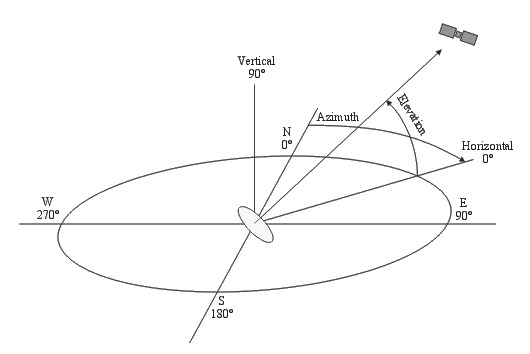
\includegraphics{images/Elevation_and_azimuth_angle.jpg}
\newpage
\Large
Wave number
\normalsize
This defines the constant $k$ in terms of wavelength $\lambda$ as the wavelength is the distance on the
x-axis before the wave repeats itself. Thus, $k = 2\pi/\lambda$ is referred to as the
wave number.\cite{Fuller1995}\\\\
\Large
Transfer function
\normalsize
refers to the rule by which an environment affects a signal.\cite{Regulinski1962}\\\\
\Large
Harmonics
\normalsize
is a function that satisfies Laplace's equation:\\
\begin{equation}
    \nabla ^2f=0
\end{equation}\\
\Large
Spherical Harmonics
\normalsize
are an infinite set of harmonic functions defined on the sphere. They arise from solving the angular portion of Laplace's equation in spherical coordinates using separation of variables\cite{Atkinson2012}


\section{Wave equation}
\subsection{Standard wave equation}
The wave standard equation is defined by
\begin{equation}
    \frac{\delta ^2 u}{\delta t^2} = c^2 \frac{\delta ^2 u}{\delta x^2}
\end{equation}
with $u$ being the wave's function\\
and $c$ the speed of the wave.
\subsection{Spherical harmonics-based wave equation}
The spherical harmonics-based wave equation solution decomposes any homogeneous incident wave field $v(\textbf{x},k)$ observed at $x$ into
\begin{equation}
    v(\textbf{x},k) = \sum_{u=0}^\infty \sum_{m=-u}^u\beta_{um}(k)j_u(kr)\Upsilon_{um}(\Phi_x,\Psi_x),
\end{equation}
where $j_u(.)$ is the spherical Bessel function of order $u$ and $\Upsilon_{um}(.)$ denotes the spherical harmonics.\cite{Zhang2019}
\subsubsection{Bessel function}

\subsubsection{Spherical harmonics}